\documentclass[a4paper,12pt]{article}
\usepackage{imakeidx}
\usepackage[utf8]{inputenc}
\makeindex
\usepackage{amsmath}
\usepackage{mathtools}
\usepackage{tikz}
\usepackage{graphicx}
\usepackage[dvipsnames]{xcolor}
\usepackage{amssymb}
\usepackage[a4paper,includeheadfoot,margin=3cm]{geometry}
\usepackage[slovene] {babel}

\begin{document}
\thispagestyle{empty}
\begin{center}
	
\begin{center}
	\normalsize
	UNIVERZA V LJUBLJANI
	
	FAKULTETA ZA MATEMATIKO IN FIZIKO
	
	Oddelek za matematiko
\end{center}
\vspace{6cm}
	\vspace{1.5cm}
	{\Large \bfseries Random lines
		\vspace{0.1cm}} \\  
        \vspace{0.3cm}{\normalsize FINANČNI PRAKTIKUM}\\
	\vspace{0.5cm} {\normalsize Avtorici: Matea Naumovska, Andreja Sitar}
	\vspace{0.2cm} \\
        \vspace{0.2cm}{\normalsize
        Mentorja: prof. dr. Sergia Cabello Justo, doc. dr. Janoš Vidali}\\
	\vspace{8cm}
	{\normalsize Ljubljana, Januar 2023}
\end{center}
\tableofcontents
\newpage
\section{Navodila}	
V ravnini lahko premico predstavimo na več načinov. Za stohastično geometrijo je priročno, da premico $l$ parametriziramo s parom ($p$,$\theta$), kjer je $p$ razdalja od izvora do premice, $\theta$ pa kot, ki ga premica oklepa z $x$ osjo. 
Naj bosta $C$ in $C'$ konveksna objekta v ravnini, kjer velja da $C'$ leži v notranjosti $C$. Želimo analizirati verjetnost, da naključna premica, ki seka $C$, seka tudi $C'$.
Premice izbiramo enakomerno naključno glede na zgoraj opisano parametrizacijo. 
\section{Formalno reševanje}
Ta problem se rešuje s pomočjo že znanega problema Buffonove igle. Premico v ravnini bomo parametrizirali s parom ($p$,$\theta$), kjer je $p$ razdalja od izvora do premice, $\theta$ pa kot, ki ga premica oklepa z $x$ osjo. 
\begin{figure}[h!]
	\begin{center}
		\includegraphics[width=4cm]{param.jpg}
            \caption{Primer premice podane s parom ($p$,$\theta$)}
	\end{center}
\end{figure}
\\
Torej je enačba premice enaka $$x\cos{\theta}+y\sin{\theta}-d=0.$$
Mero množice $Y$ premic lahko definiramo z integralom $$m(Y)=\int_{Y} f(p,\theta) dY=\iint f(p,\theta)\,dp\,d\theta,$$kjer je $f(p,\theta)$ konstantna funkcija, ker vemo, da je ta mera nespremenljiva za toge premike ravnine.\\
\\
Naj bo $X$ množica vseh afinih premic v $\mathbb{R}^2$ in $Z_1$ naključna spremenljivka, ki šteje presečišča naključne premice z odsekom dolžine $L_1$. Potem je integral $$\int_{X} Z_1 dX $$ odvisen le od $L_1$. Ker $Z_1$ zavzema le vrednosti 0 ali 1, je ta integral enak meri množice vseh
premic, ki sekajo dani segment ($\int_{X} Z_1 dX=m(X)$). Ker je vrednost integrala odvisna le od $L_1$, to vrednost označimo z $g(L_1).$ \\
Sedaj lahko ponovimo utemeljitev za rešitev problema Buffonove igle: Število presečišč naključno izbrane premice s fiksno mnogokotno črto, sestavljeno iz odsekov dolžin $L_1$, $L_2$,... je
$$\int_{X} (Z_1+Z_2+\cdots) dX=g(L_1+L_2+\cdots).$$
To se zaradi linearnosti integralov ujema z 
$$\int_{X} Z_1 dX + \int_{X} Z_2 dX+\cdots=g(L_1)+g(L_2)+\cdots,$$
iz česar sklepamo, da obstaja konstanta $r$, taka da $$g(L)=rL.$$
Če je $C$ konveksna krivulja v ravnini dolžine $L$ in $Z_C$ označuje naključno spremenljivko, ki šteje presečišča $C$ z naključno premico, potem dobimo $$\int_{X} Z_C dX=rL.$$
Naj bosta zdaj sta $K_1$ in $K_2$ kompaktni konveksni množici v ravnini z nepraznima notranjostma z mejnima krivuljama $C_1 =\partial K_1$ in $C_2 =\partial K_2$ dolžin $L_1$ in $L_2$. Sledi $$\int_{X} Z_{C_i} dX=rL_i,\hspace{1cm} i=1,2.$$
Ker sta množici $K_i$ konveksni, premica seka $C_i$ bodisi dvakrat bodisi nikoli. Naključni spremenljivki $Z_{C_i}$ torej zavzameta le vrednosti 2 in 0 in velja  $$\int_{X} Z_{C_i} dX=2L_i,\hspace{1cm} i=1,2.$$
Odgovor na vprašanje, s kakšno verjetnostjo naključna premica seka konveksno množico $K_1$, če je $K_1 \subseteq K_2$ in že vemo, da premica seka množico $K_2$ je $$\frac{\int_{X} Z_{C_q} dX}{\int_{X} Z_{C_2} dX}=\frac{2L_1}{2L_2}=\frac{L_1}{L_2}=\frac{obseg(K_1)}{obseg(K_2)}.$$
\\
V našem primeru je torej 
$$P(premica\ l\ seka\ C'\ |\ premica\ l\ seka\ C)=\frac{obseg(C')}{obseg(C)}.$$
\section{Reševanje s pomočjo programa in simulacij}
Napisali sva program, ki najprej iz 15 poljubnih točk generira poljuben konvenksni objekt $C$. Nato iz nabora teh točk izvzame tiste, ki se nahajajo v ovojnici $C$ in iz preostalih generira nov podobjekt $C'$, torej $C' \subseteq C$. To delamo s pomočjo funkcij $random$ in $ConvexHull$.
\begin{figure}[h!]
	\begin{center}
		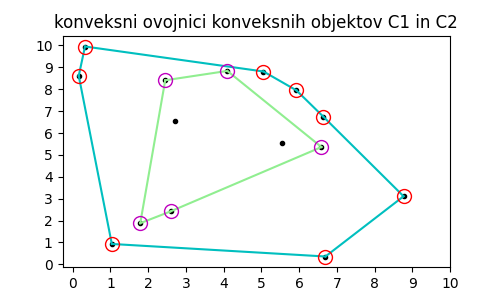
\includegraphics[width=9cm]{Figure_4.png}
		\caption{Primer koveksnih ovojnic $C=C1$ in $C'=C2$.}
	\end{center}
\end{figure}\\
Pogledali sva si, če  premice, ki gredo skozi naključno izbrane točke v notranjosti $C$ (torej ne nujno v notranjosti $C'$) - torej zagotovo sekajo $C$, sekajo tudi $C'$.
Da sva preverili sekanje sva si pomagali z determinantami, in sicer sva izbrali dve točki na premici $p_1$ = ($x_1$, $y_1$) in $p_2$ = ($x_2$, $y_2$), ena znotraj objekta $C$ in ena izven, ter dve sosednji ogljišči $C'$ $p_3$ = ($x_3$, $y_3$) in $p_4$ = ($x_4$, $y_4$).
\begin{center}
    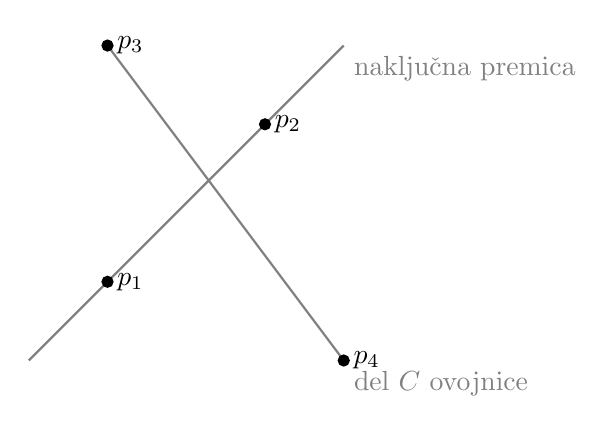
\begin{tikzpicture}
        \draw[gray, thick] (-2,1) -- (1,-3) node[anchor=north west] {del $C$ ovojnice};
        \draw[gray, thick] (-3,-3) -- (1,1) node[anchor=north west] {naključna premica};
        \filldraw[black] (-2,1) circle (2pt) node[anchor=west]{$p_3$};
        \filldraw[black] (1,-3) circle (2pt) node[anchor=west]{$p_4$};
        \filldraw[black] (-2,-2) circle (2pt) node[anchor=west]{$p_1$};
        \filldraw[black] (0,0) circle (2pt) node[anchor=west]{$p_2$};
    \end{tikzpicture}
\end{center}
Označimo $$\Lambda(p_1,p_2,p_3) = \begin{vmatrix}
     1 & x_{1} & y_{1}\\ 
     1 & x_{2} & y_{2}\\
     1 & x_{3} & y_{3} 
\end{vmatrix}$$. Vemo, da se naključna premica, na kateri sta točki $p_1$ in $p_2$, in daljica $\overrightarrow{\rm p_3p_4}$ sekata $\Leftrightarrow$ $[\Lambda(p_1,p_2,p_3)\cdot\Lambda(p_1,p_2,p_4)]\leq 0.$ \\
S pomočjo te informacije lahko za vsako premico preverimo, če seka $C'$.
Verjetnost, da premica seka $C'$, če vemo, da seka $C$, je v tem primeru dana s koeficientom $$\frac{število\ premic,\ ki\ sekajo\ C'}{število\ premic,\ ki\ jih\ gledamo}.$$
Ogledali sva si primere različnega števila premic in pogledali ujemanje z zgoraj izpeljano formulo $$P(premica\ l\ seka\ C'\ |\ premica\ l\ seka\ C)=\frac{obseg(C')}{obseg(C)}.$$

\begin{figure}[h!]
	\begin{center}
		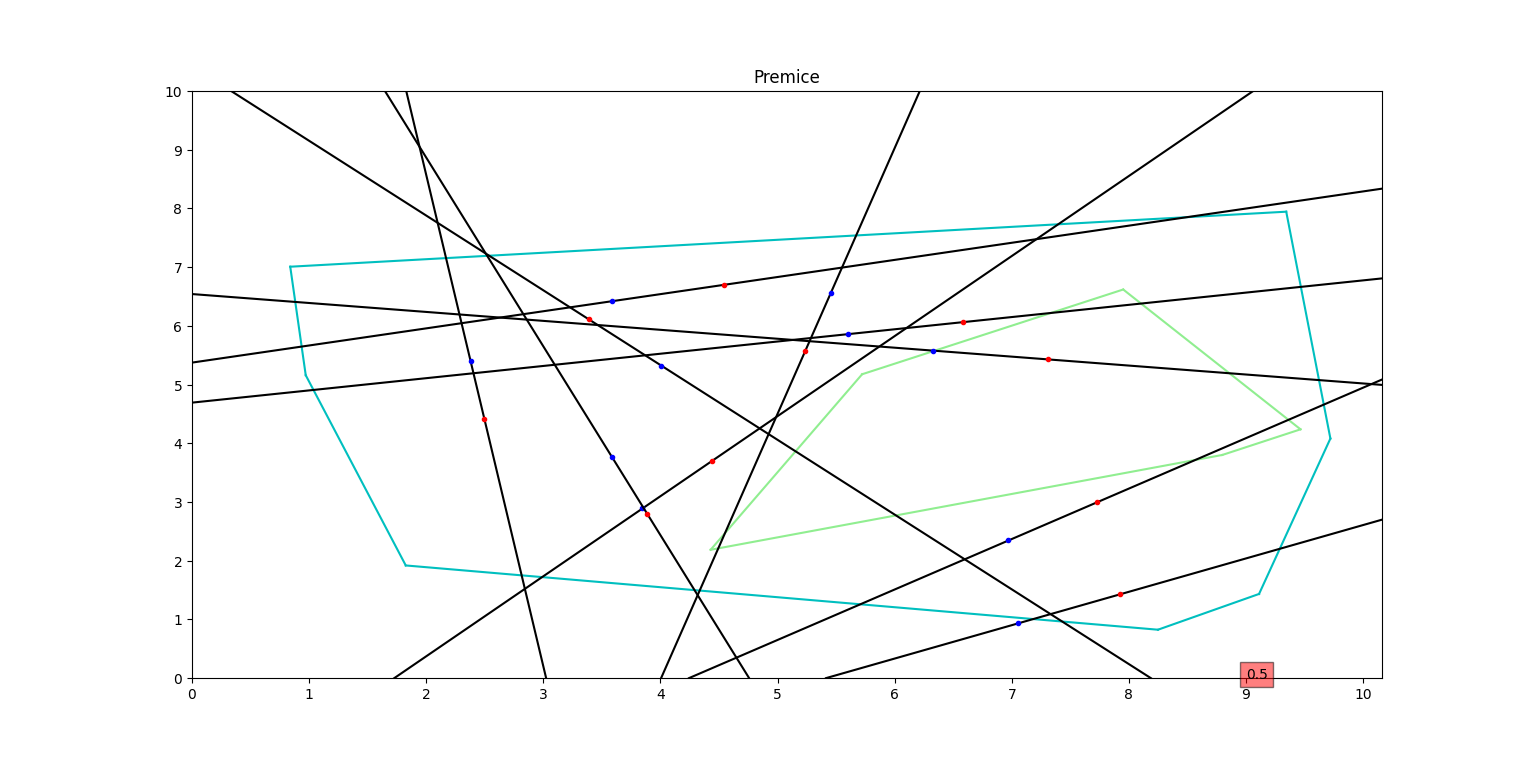
\includegraphics[width=9cm]{Figure_5.png}
		\caption{Primer za 10 premic.}
	\end{center}
\end{figure}\\

\begin{table}[h!]
    \begin{center}
      \label{tab:table1}
      \begin{tabular}{l|r|u|v} % <-- Alignments: 1st column left, 2nd middle and 3rd right, with vertical lines in between
        \textbf{št. premic} & \textbf{št. premic, ki sekajo oba} & \textbf{$P$ po programu} & \textbf{$P$ po formuli}\\
        \hline
        5 & 3 & 0.6 & 0.6567108861061377 \\
        10 & 8 & 0.8 & 0.6965224589290716 \\
        20 &  17 & 0.85 & 0.5550093283090112\\
        100 &  92 & 0.92 & 0.7892159960747438\\
        1000 &  848 & 0.848 & 0.7326084423923283\\
        \hline
      \end{tabular}
    \end{center}
  \end{table}
Vidimo lahko, da je s povečevanjem števila premic razlika med razultatoma vedno manjša.

\begin{thebibliography}{9}
\bibitem{geometric} L.A. Santalo. \textit{Integral geometry and geometric probability}. Addison-Wesley Publishing Co., Reading, Mass.-London-Amsterdam, pp. 12-33, 1976.
\bibitem{schuster} Franz Schuster. \textit{Integralgeometrie}. (German): pp. 3–6, 2017.
\bibitem{adamwebsite} Adam G. Weyhaupt: The Cauchy-Crofton Formula, 2003,\\\texttt{https://www.siue.edu/~aweyhau/project.html}
\end{thebibliography}
\end{document}
